\documentclass[a4paper]{article}
\usepackage[utf8]{inputenc}

\usepackage{amsmath}
\usepackage{amssymb}
\usepackage{amsthm}

\usepackage{graphicx}

\usepackage{mdframed}
\usepackage{proof}

\renewcommand{\qed}{\hfill\ensuremath{\square}}

\newenvironment{claim}[1]{\par\noindent\underline{Claim:}\space#1}{}
\newenvironment{claimproof}[1]{\par\noindent\underline{Proof:}\space#1}{\qed}

\newcommand{\optimization}[2]{
	\[
		\begin{array}{rcl}
			#1 & \Rightarrow & #2
		\end{array}
	\]
}

\title{G2C: an optimizing transcompiler for probabilistic programming languages}
\author{Robert Brignull}
\date{ }

\begin{document}

\maketitle

%     ##       #### ##    ## ######## ######    ##### 
%    ###   ##   ##  ###   ##    ##    ##   ##  ##   ##
%     ##   ##   ##  ####  ##    ##    ##   ##  ##   ##
%     ##        ##  ## ## ##    ##    ######   ##   ##
%     ##   ##   ##  ##  ####    ##    ##  ##   ##   ##
%     ##   ##   ##  ##   ###    ##    ##   ##  ##   ##
%    ####      #### ##    ##    ##    ##    ##  ##### 

\section{Introduction}



%     ##        ## 
%    ###       ### 
%     ##        ## 
%     ##        ## 
%     ##        ## 
%     ##   ##   ## 
%    ####  ##  ####

\subsection{The purpose of the project}

Talk about how there a many different probabilistic programming languages.

A lot are both functional and interpreted as this makes them easy to code in and easy to implement, but it lessens their performance.

Prob-C is the opposite, being based on C it is more difficult to code in but by being a compiled language and highly multi-threaded it has good performance.

The purpose of this project is to create a transcompiler from a functional probabilistic programming language into Prob-C.

If any optimizations can be done along the way, either probabilistic or not, then that is even better.



%     ##        ###### 
%    ###       ##    ##
%     ##            ###
%     ##          ###  
%     ##        ###    
%     ##   ##  ##      
%    ####  ##  ########

\subsection{How this was achieved}

Because both my source language and Prob-C handle sampling and observing in a very similar way, the bulk of the compiler is very standard.

It first transforms into continuation passing style, then adds closures to functions and hoists them to the top level, before outputting C code.

It performs some non-probabilistic optimizations such as identifier reassignment and constant expression calculation.

It performs probabilistic optimizations such as merging multiple samples from one distribution family into one sample, and potentially removing observes when it forms a conjugate prior.



%     ######       ######     ##     #####  ##   ##  #####   ######    #####  ##   ## ##    ## ###### 
%    ##    ##  ##  ##   ##   ####   ##   ## ##  ##  ##   ##  ##   ##  ##   ## ##   ## ###   ## ##   ##
%         ###  ##  ##   ##  ##  ##  ##      ## ##   ##       ##   ##  ##   ## ##   ## ####  ## ##   ##
%       ###        ######  ##    ## ##      ####    ##       ######   ##   ## ##   ## ## ## ## ##   ##
%     ###      ##  ##   ## ######## ##      ## ##   ##  #### ##  ##   ##   ## ##   ## ##  #### ##   ##
%    ##        ##  ##   ## ##    ## ##   ## ##  ##  ##   ##  ##   ##  ##   ## ##   ## ##   ### ##   ##
%    ########      ######  ##    ##  #####  ##   ##  #####   ##    ##  #####   #####  ##    ## ###### 

\section{Background}



%     ######        ## 
%    ##    ##      ### 
%         ###       ## 
%       ###         ## 
%     ###           ## 
%    ##        ##   ## 
%    ########  ##  ####

\subsection{Probabilistic programming}

A probabilistic programming language is just like a normal one except with the ability to easily draw from random distributions and to condition the program execution on other random variables.

Usually a probabilistic programming language is based on an existing language rather than being a completely new one, examples include: Venture (Scheme), Anglican (Scheme), IBAL (OCaml), Infer.NET (.NET), PSQL (SQL), FACTORIE (Scala), Alchemy (C++), Church (Scheme), Stan (none).

Probabilistic programming languages do their inference in one of a few different ways, including Markov Chain Monte Carlo (MCMC) and Sequential Monte Carlo (SMC) algorithms.

The applications of probabilistic programming are diverse, anything that requires estimating a distribution given prior beliefs and conditioned on some observed data. It can be used in machine learning, financial modeling, etc.



%     ######        ###### 
%    ##    ##      ##    ##
%         ###           ###
%       ###           ###  
%     ###           ###    
%    ##        ##  ##      
%    ########  ##  ########

\subsection{Anglican and Prob-c}

Anglican and Prob-C are the two languages we'll be concerned with most, Anglican because it's what I've based my source language on, and Prob-C because it is the target language of my compiler.

Anglican is based on the Venture modeling language which is itself based on Scheme. Anglican is effectively one language embedded inside another, specifically it is build from a sequence of the commands Assume, Observe and Predict, each of which can contain expressions which come from a functional subset of Scheme.

Prob-C on the other hand is based on full C rather than a subset, in fact the only difference is the addition of a library of sampling functions, two extra functions to observe and predict, and a macro which redefines the main function. So Prob-C has all the power of C. Unlike almost all other probabilistic programming languages, Prob-C is unsafe in the sense that it is possible to create programs which make no sense statistically, for this reason as well as C's unfriendliness it is not recommended to code in Prob-C directly.



%     ######        ##### 
%    ##    ##      ##   ##
%         ###           ##
%       ###         ##### 
%     ###               ##
%    ##        ##  ##   ##
%    ########  ##   ##### 

\subsection{Bayesian probability}

Bayesian probability revolves around the idea of conditional probability, that is having some prior belief about an event and then estimating it's probability once you've observed that some other event happened.

The central theorem is Bayes' theorem \(p(A | B) = \dfrac{p(A \land B)}{p(B)}\)



%     #####        #####   #####  ##      ## ######  #### ##     ####### ######  
%    ##   ##  ##  ##   ## ##   ## ###    ### ##   ##  ##  ##     ##      ##   ## 
%         ##  ##  ##      ##   ## ####  #### ##   ##  ##  ##     ##      ##   ## 
%     #####       ##      ##   ## ## #### ## ######   ##  ##     ######  ######  
%         ##  ##  ##      ##   ## ##  ##  ## ##       ##  ##     ##      ##  ##  
%    ##   ##  ##  ##   ## ##   ## ##      ## ##       ##  ##     ##      ##   ## 
%     #####        #####   #####  ##      ## ##      #### ###### ####### ##    ##

\section{The compiler}



%     #####        ## 
%    ##   ##      ### 
%         ##       ## 
%     #####        ## 
%         ##       ## 
%    ##   ##  ##   ## 
%     #####   ##  ####

\subsection{The source language}

For this project I had to invent my own toy language, I chose to base it on Anglican but with some extra type information to make compilation easier.

** Small example program **

Without this extra type information, when translated to C all variables would have to be data-structures rather than native types, this would largely eliminate the benefit of transforming to a compiled language.

** BNF of G **



%     #####        ###### 
%    ##   ##      ##    ##
%         ##           ###
%     #####          ###  
%         ##       ###    
%    ##   ##  ##  ##      
%     #####   ##  ########

\subsection{Typing the source language}

Typing the source language is very easy, all the information is there and only minimal inference has to be done.

We know the types of simple values such as numbers and booleans.

For all built-in functions (eg. +, -, and, or) we know their type or in the case of = can give them one based on their argument types. Then we just check that the types of the arguments match the types of the formal parameters.

For if expressions we check that the test is a boolean type and that both of the branches have the same type.

For lambdas the user must specify the parameter types and return type, so we just check that the actual type of the body matches the return type they gave. We have to do a little bit of extra work to deal with recursive functions, this is the reason why function return types must be specified.

For an observe, check that the outer expression of the first argument is a probabilistic primitive. This is a restriction of the sampling method and hence of the language.



%     #####        ###### 
%    ##   ##      ##    ##
%         ##            ##
%     #####        ###### 
%         ##            ##
%    ##   ##  ##  ##    ##
%     #####   ##   ###### 

\subsection{Making ids unique}

At this point we change all ids to be unique, that is so that whenever two ids are the same then they refer to the same variable.

This means that for the rest of the compilation we do not have to worry about the scope of variables at all.



%     #####           ### 
%    ##   ##         #### 
%         ##        ## ## 
%     #####        ##  ## 
%         ##      ########
%    ##   ##  ##       ## 
%     #####   ##       ## 

\subsection{Into continuation passing style}

The first step is to transform into continuation passing style.

The main difference is that now functions do not return values but instead take as another parameter a function to call when they're done with the value they would have returned.

The exception to this is built-in primitives which we assume can be done atomically by the target language and hence they can be calculated directly and stored into variables.

It is this step that is the defining transition from a functional to an imperative language.



%     #####       ########
%    ##   ##      ##      
%         ##      ##      
%     #####        ###### 
%         ##            ##
%    ##   ##  ##  ##    ##
%     #####   ##   ###### 

\subsection{Closure conversion and hoisting}

What we want to do in this step is to lift all functions to the top level of the program, as they must be defined that way in a C program. The problem is that functions may reference variables defined outside of their scope.

Closure conversion concerns working out which are the variables used by a function are free variables and which are present in the arguments or defined by let expressions within that function.

The effect of this is almost to add more arguments to the function so that it has no free variables, in practice however we keep separate the original arguments and the new arguments are formed into one package, a closure or bundle.

Once this has been done all function definitions can be lifted to the top level of the program. Whenever a function would have been defined we instead instantiate a data structure containing the name of the function and the values of all variables it references formed into a closure.



%     #####           ## 
%    ##   ##         ##  
%         ##        ##   
%     #####        ##### 
%         ##      ##   ##
%    ##   ##  ##  ##   ##
%     #####   ##   ##### 

\subsection{Outputting C code}

We need to output valid C code, including struct definitions and any extra library functions used.

Mostly the translation here is obvious and direct, only difficult point is to make sure all structs and functions are defined before they are described to allow full recursion.

One important point is we don't need to worry about memory management at all, which simplifies like tremendously. This is because each run of the program happens within its own thread and when it ends the operating system will release all memory it owns. Because each thread is short lived and doesn't use much memory individually, the memory usage of the program is low and does not grow over time.



%        ###        #####  ######  ######## #### ##      ## #### ########    ##    ######## ####  #####  ##    ##  ##### 
%       ####   ##  ##   ## ##   ##    ##     ##  ###    ###  ##       ##    ####      ##     ##  ##   ## ###   ## ##     
%      ## ##   ##  ##   ## ##   ##    ##     ##  ####  ####  ##      ##    ##  ##     ##     ##  ##   ## ####  ## ##     
%     ##  ##       ##   ## ######     ##     ##  ## #### ##  ##     ##    ##    ##    ##     ##  ##   ## ## ## ##  ##### 
%    ########  ##  ##   ## ##         ##     ##  ##  ##  ##  ##    ##     ########    ##     ##  ##   ## ##  ####      ##
%         ##   ##  ##   ## ##         ##     ##  ##      ##  ##   ##      ##    ##    ##     ##  ##   ## ##   ###      ##
%         ##        #####  ##         ##    #### ##      ## #### ######## ##    ##    ##    ####  #####  ##    ##  ##### 

\section{Optimizations}

Although just having a compiler from a high level probabilistic language into a lower lever one such as Prob-C would be a good enough project in itself, there is potential for massive increases in both performance and the quality of samples though a combination of a few simple optimizations.

All the optimizations described here are performed immediately after CPS transformation. In this stage the syntax is in a good balance of simple and expressive, for example all expressions have been split up so we only calculate one primitive or application at a time, but lambdas are still in-line and so we don't have to worry about variable scope as much. It is however still often useful to know the full history of a variable, that is exactly how it was calculated rather than just the last step, so we calculate this history before doing any optimizations and rebuild the information after each one.



%        ###        ## 
%       ####       ### 
%      ## ##        ## 
%     ##  ##        ## 
%    ########       ## 
%         ##   ##   ## 
%         ##   ##  ####

\subsection{Non-probabilistic optimizations}

We do some standard non-probabilistic optimizations. None of these are technically necessary for the rest of the optimizations to work and some would be performed by the C compiler anyway. They still make our life a little easier however so that is why they are included here.



%        ###         ##        ## 
%       ####        ###       ### 
%      ## ##         ##        ## 
%     ##  ##         ##        ## 
%    ########        ##        ## 
%         ##   ##    ##   ##   ## 
%         ##   ##   ####  ##  ####

\subsubsection{Constant expression calculation}

When the arguments to a primitive such as plus or times are all constant, we can easily calculate what the answer should be and set the id equal to that rather than applying a primitive.

For example we could do the following optimization
\optimization{
	\begin{array}{l}
		\texttt{let x = prim + 2 5 in} \\
		\texttt{...}
	\end{array}
}{
	\begin{array}{l}
		\texttt{let x = 7 in} \\
		\texttt{...}
	\end{array}
}
This can be extended to the case when only some of the arguments are constant, now we can't remove the whole primitive application but we can reduce the number of arguments and hence the complexity of it.

For example we could do the following optimization
\optimization{
	\begin{array}{l}
		\texttt{let x = ... in} \\
		\texttt{let y = prim + x 2 5 in} \\
		\texttt{...}
	\end{array}
}{
	\begin{array}{l}
		\texttt{let x = ... in} \\
		\texttt{let y = prim + x 7 in} \\
		\texttt{...}
	\end{array}
}
We can optimize all of the following when at least some of the arguments are constant:
\begin{center}
	\texttt{+}, \texttt{-}, \texttt{*}, \texttt{/}, \texttt{eq}, \texttt{neq}, \texttt{<}, \texttt{>}, \texttt{<=}, \texttt{>=}, \texttt{and}, \texttt{or}, \texttt{not}
\end{center}
This sort of optimization would definitely be performed by any half decent C compiler, so we are not actually improving the performance of the final compiled program by doing this. The reason for doing it is it reduces the size and complexity of the generated Prob-C code greatly, therefore making other stages of compilation faster and easier and also making it easier for a human to scan and understand the outputted Prob-C code.



%        ###         ##        ###### 
%       ####        ###       ##    ##
%      ## ##         ##            ###
%     ##  ##         ##          ###  
%    ########        ##        ###    
%         ##   ##    ##   ##  ##      
%         ##   ##   ####  ##  ########

\subsubsection{Merging multiple arithmetic expressions}

Another thing we can do with arithmetic expressions is to merge ones of the same sort together.

For example we could do the following optimization
\optimization{
	\begin{array}{l}
		\texttt{let x = ... in} \\
		\texttt{let y = prim + x 5 in} \\
		\texttt{let z = prim + y 8 in} \\
		\texttt{let w = prim + z -4 in} \\
		\texttt{...}
	\end{array}
}{
	\begin{array}{l}
		\texttt{let x = ... in} \\
		\texttt{let w = prim + x 9 in} \\
		\texttt{...}
	\end{array}
}
This is a case that comes up in compiled programs surprisingly often, especially after other optimizations, so by optimizing it away we reduce the final complexity of the Prob-C.

Again this optimization would likely be performed by the C compiler anyway so the final compiled program is unchanged.



%        ###         ##        ###### 
%       ####        ###       ##    ##
%      ## ##         ##             ##
%     ##  ##         ##        ###### 
%    ########        ##             ##
%         ##   ##    ##   ##  ##    ##
%         ##   ##   ####  ##   ###### 

\subsubsection{Removing let expressions where the id is not used}

A very simple optimization is to remove any let expression where the variable being assigned to is never used later on in the program.

This optimization doesn't do much on its own, as the user is unlikely to have written a program that doesn't use one of its variables, but almost all of the other optimizations we do here will leave orphaned variables that this process will clean up.

This is an optimization that a C compiler potentially would not perform. This is because C is a language with side effects so just because a variable is never used does not mean that the process of calculating it did not change program state. In our language however variables are immutable and there is no state so it is safe to remove the unused variable.



%        ###         ##           ### 
%       ####        ###          #### 
%      ## ##         ##         ## ## 
%     ##  ##         ##        ##  ## 
%    ########        ##       ########
%         ##   ##    ##   ##       ## 
%         ##   ##   ####  ##       ## 

\subsubsection{Removing let expressions where an id is assigned to another id}

Another very simple optimization is to remove a variable when it is assigned to the value of another variable. We then change all references to the removed variable in the rest of the program to the variable it was assigned to.

For example we could do the following optimization
\optimization{
	\begin{array}{l}
		\texttt{let x = ... in} \\
		\texttt{let y = x in} \\
		\texttt{let z = prim + y 1 in}\\
		\texttt{...}
	\end{array}
}{
	\begin{array}{l}
		\texttt{let x = ... in} \\
		\texttt{let z = prim + x 1 in}\\
		\texttt{...}
	\end{array}
}
This optimization is admittedly rather inconsequential, but we include it anyway.



%        ###         ##       ########
%       ####        ###       ##      
%      ## ##         ##       ##      
%     ##  ##         ##        ###### 
%    ########        ##             ##
%         ##   ##    ##   ##  ##    ##
%         ##   ##   ####  ##   ###### 

\subsubsection{Removing trivial continuations}

The final non-probabilistic optimization we do it to remove trivial functions which are equivalent to another function. The place where this happens a lot is continuations generated from the translation into CPS.

For example we could do the following optimization
\optimization{
	\begin{array}{l}
		\texttt{let f = lambda x y z -> g x y z in} \\
		\texttt{...}
	\end{array}
}{
	\begin{array}{l}
		\texttt{let f = g in} \\
		\texttt{...}
	\end{array}
}
This will then of course be removed on the next pass as it is an id assigned to another id.

This optimization could be moderately important for performance. Although a decent C compiler will inline a small function such as the above and hence remove the extra application, after the other transformations that G2C performs it will not be simple, so removing it at this stage will greatly simplify later stages of compilation.



%        ###        ###### 
%       ####       ##    ##
%      ## ##            ###
%     ##  ##          ###  
%    ########       ###    
%         ##   ##  ##      
%         ##   ##  ########

\subsection{Samples}

One of the things we'd like to do is to reduce the number of samples as some of them can be quite costly, and more importantly improve the quality of the ones we do. By this I mean we'd like to have a high level of mixing, so we need to make fewer runs of the program before the output has converged enough towards to the correct output.



%        ###        ######         ## 
%       ####       ##    ##       ### 
%      ## ##            ###        ## 
%     ##  ##          ###          ## 
%    ########       ###            ## 
%         ##   ##  ##        ##    ## 
%         ##   ##  ########  ##   ####

\subsubsection{Merging samples}

One way we can improve performance is to reduce the number of samples as some of them can be moderately costly to perform. The ideal case for this optimization is shown below.
\[
	\begin{array}{l}
		\texttt{[assume x\_1 (normal m\_1 b\_1)]} \\
		\texttt{...} \\
		\texttt{[assume x\_n (normal m\_n b\_n)]} \\
		\texttt{[assume y (+ x\_1 ...\ x\_n)]}
	\end{array}
\]
The general form is where we make many samples and perform some function on them, we then use that function output and never use the individual samples anywhere else.

Assuming that none of the \texttt{x\_i} are used anywhere else then the above can be optimized into the following
\[
	\texttt{[assume y (normal (+ m\_1 ...\ m\_n) (+ b\_1 ...\ b\_n))]}
\]
We can even perform this optimization in the case where some of the \texttt{x\_i}s are used again. If only \texttt{x\_1} were used elsewhere then we could optimize to the following
\[
	\begin{array}{l}
		\texttt{[assume x\_1 (normal m\_1 b\_1)]} \\
		\texttt{[assume t (normal (+ m\_2 ...\ m\_n) (+ b\_2 ...\ b\_n))]} \\
		\texttt{[assume y (+ x\_1 t)]}
	\end{array}
\]
Although less of an optimization we have still reduced the number of samples.

There are many cases where we can apply this optimization, some of which I have listed below. I have only included here a few for the normal distribution, but the optimization can be applied to many other distributions and operations.

\begin{center}
	\resizebox{\textwidth}{!}{%
	\begin{tabular}{lcl}
		Before optimization && After optimization \\[2mm]
		\hline \\[-2mm]

		\(\begin{array}{l}
				\texttt{[assume x\_1 (normal m\_1 b\_1)]} \\
				\texttt{...} \\
				\texttt{[assume x\_n (normal m\_n b\_n)]} \\
				\texttt{[assume y (+ x\_1 ...\ x\_n)]}
			\end{array}\)
		&\(\Rightarrow\)&
		\texttt{[assume y (normal (+ m\_1 ...\ m\_n) (+ b\_1 ...\ b\_n))]} \\[15mm]

		\(\begin{array}{l}
				\texttt{[assume x\_1 (normal m\_1 b\_1)]} \\
				\texttt{...} \\
				\texttt{[assume x\_n (normal m\_n b\_n)]} \\
				\texttt{[assume y (- x\_1 ...\ x\_n)]}
			\end{array}\)
		&\(\Rightarrow\)&
		\texttt{[assume y (normal (- m\_1 ...\ m\_n) (+ b\_1 ...\ b\_n))]}

	\end{tabular}}
\end{center}
I will also prove the correctness of the first example.

\begin{mdframed}
	\begin{claim}
	  The sum of independent normally distributed variables is normally distributed.
	\end{claim}
	\begin{claimproof}
	  The easiest way to do this is using characteristic functions. For a random variable \(X\) this is

	  \[\varphi_X(t) = E(e^{itX})\]
	  The characteristic function of a normal distribution with mean \(\mu\) and variance \(\sigma^2\) is

	  \[\varphi(t) = \exp(i t \mu - \frac{\sigma^2 t^2}{2})\]
	  The characteristic function of the sum of two independent random variables \(X\) and \(Y\) is the product of their separate characteristic functions. Hence if \(X\) and \(Y\) are both normally distributed with means and variances \(\mu_X\), \(\mu_Y\) and \(\sigma_X^2\), \(\sigma_Y^2\) respectively, then

  	\begin{align*}
  		\varphi_{X+Y}(t)
  		& = \varphi_X(t) \varphi_Y(t) \\
  		& = \exp\left(i t \mu_X - \frac{\sigma_X^2 t^2}{2}\right) \exp\left(i t \mu_Y - \frac{\sigma_Y^2 t^2}{2}\right) \\
  		& = \exp\left(i t (\mu_x + \mu_Y) - \frac{(\sigma_X^2 + \sigma_Y^2) t^2}{2}\right)
  	\end{align*}
	  Which is the characteristic function of a normal distribution with mean \(\mu_X + \mu_Y\) and variance \(\sigma_X^2 + \sigma_Y^2\).

	  From here if we have \(n\) independent normally distributed random variables \(X_i \sim N(\mu_i, \sigma_i^2)\) then we proceed by induction using the above to get that

	  \[\sum_{i=1}^n X_i \sim N(\sum_{i=1}^n \mu_i, \sum_{i=1}^n \sigma_i^2)\]
	\end{claimproof}
\end{mdframed}



%        ###        ######         ###### 
%       ####       ##    ##       ##    ##
%      ## ##            ###            ###
%     ##  ##          ###            ###  
%    ########       ###            ###    
%         ##   ##  ##        ##   ##      
%         ##   ##  ########  ##   ########

\subsubsection{Doing arithmetic on samples}

Another thing we can do is merge some arithmetic operations into the sample, as shown below. Although not very helpful at all on its own, the hope is it would allow us to later merge more samples as in the previous optimization. With these two together we can merge any linear combination of samples into only one sample.

Here are some examples of the sort of optimizations we could do. However note that there are many others of this form that could be done and not just involving the normal distribution.

\begin{center}
	\resizebox{\textwidth}{!}{%
	\begin{tabular}{lcl}
		Before optimization && After optimization \\[2mm]
		\hline \\[-2mm]

		\(\begin{array}{l}
				\texttt{[assume x (normal m b)]} \\
				\texttt{[assume y (+ x r)]}
			\end{array}\)
		&\(\Rightarrow\)&
		\texttt{[assume y (normal (+ m r) b)]} \\[10mm]

		\(\begin{array}{l}
				\texttt{[assume x (normal m b)]} \\
				\texttt{[assume y (* x s)]}
			\end{array}\)
		&\(\Rightarrow\)&
		\texttt{[assume y (normal (* m s) (* b s s))]}

	\end{tabular}}
\end{center}



%        ###        ######        ###### 
%       ####       ##    ##      ##    ##
%      ## ##            ###            ##
%     ##  ##          ###         ###### 
%    ########       ###                ##
%         ##   ##  ##        ##  ##    ##
%         ##   ##  ########  ##   ###### 

\subsubsection{Pushing samples back}

Something we can do which has the capacity to greatly improve the quality of samples made is to move samples after potentially costly observe statements. The idea is that when an observe is made that kills almost all of the particles, the ones which remain will all have been cloned from some small set and hence all samples that have been made also come from some small set. However by moving the sample after the observe, whatever happens with the cloning of particles, they will all have different values of the sample just made.

An example of what we might do is
\optimization{
	\begin{array}{l}
		\texttt{[assume x (poisson 1)]} \\
		\texttt{[assume y (normal 0 1)]} \\
		\texttt{[observe (normal x 1) 100]} \\
		\texttt{[predict y]}
	\end{array}
}{
	\begin{array}{l}
		\texttt{[assume x (poisson 1)]} \\
		\texttt{[observe (normal x 1) 100]} \\
		\texttt{[assume y (normal 0 1)]} \\
		\texttt{[predict y]}
	\end{array}
}
The only check we make when pushing samples back is whether the operation immediately following the samples uses the sampled value, if not then we move the sample past. Note that in a perfect world we'd be able to remove the observe and the value \texttt{x} completely as they have no effect on the predicted value \texttt{y}, however we do not consider this as it is hard to work out when it is safe to do.

Care must be taken when implementing this so as to not end up in a loop, for example where you are swapping two samples back and forth forever. The crucial point when implementing this therefore is to avoid just swapping with another sample.

So, in that vein, to push a sample back, scan from its position considering each statement encountered in the following manner:
\begin{itemize}
\item
	If the statement depends on the sampled value, then the sample cannot be moved back any further.

\item
	If the statement is a \texttt{let} expression defining a new variable that does not depend on the sampled value, then just ignore it and move on to the next statement.

\item
	If the statement does depend on the sampled value and is not a \texttt{let} expression, then the original sample is moved to be right after this statement. The process is then started again from the sample's new position.

\end{itemize}
This process is run repeatedly for every sample until no more changes can be made.



%        ###        ###### 
%       ####       ##    ##
%      ## ##             ##
%     ##  ##        ###### 
%    ########            ##
%         ##   ##  ##    ##
%         ##   ##   ###### 

\subsection{Merging of observe statements}

In most cases it is the observations that govern running time rather than any computation being performed, so much so that the cost of sampling and other computation is often negligible. Observations also impact on sample quality by causing the death and cloning of particles. This set of optimizations focus on merging observations together and can improve the speed of a program greatly.



%        ###        ######        ## 
%       ####       ##    ##      ### 
%      ## ##             ##       ## 
%     ##  ##        ######        ## 
%    ########            ##       ## 
%         ##   ##  ##    ##  ##   ## 
%         ##   ##   ######   ##  ####

\subsubsection{Merging observes of the same distribution}

The scenario here is that there are multiple consecutive observes of the same distribution. What we note is that it is usually the case then that their conjunction can be written in a nicer form, as a function of some selection of properties of the observed data such as the sum or the sample mean and variance.

This optimization can be applied to many different distributions, some are obvious such as multiple identical Bernoulli observes being equivalent to one binomial observe, some are more complicated such as the case of normal distributions which we will focus on.

If we have the situation
\[
	\begin{array}{l}
		\lbrack \mathsf{observe}\ (\mathsf{normal}\ m\ b)\ x_1 \rbrack \\
		\dots \\
		\lbrack \mathsf{observe}\ (\mathsf{normal}\ m\ b)\ x_n \rbrack
	\end{array}
\]
then we can show that it is equivalent to an observe that only relies on the sample mean and variance of the \(x_i\)'s. Note however that the resulting observe will not be of a normal distribution, in fact it will not be of any of the distributions that Prob-C has a primitive for.

To work out what distribution it will have, consider the joint probability density function, which can be written as a product of the individual densities as all the observations are independent. Here \(\bar{x}\) denotes the sample mean and \(s^2\) the sample variance.

\begin{flalign*}
	   & \prod_{i=1}^n \frac{1}{\sqrt{2 \pi \sigma^2}} e^{-\frac{(x_i - \mu)^2}{2 \sigma^2}} & \notag\\
	=\ & (2 \pi \sigma^2)^{-\frac{n}{2}} e^{-\frac{1}{2 \sigma^2} \sum_{i=1}^n (x_i - \mu)^2} \notag\\
	=\ & (2 \pi \sigma^2)^{-\frac{n}{2}} e^{-\frac{1}{2 \sigma^2} \sum_{i=1}^n ((x_i - \bar{x}) - (\mu - \bar{x}))^2} \notag\\
	=\ & (2 \pi \sigma^2)^{-\frac{n}{2}} e^{-\frac{1}{2 \sigma^2} (\sum_{i=1}^n (x_i - \bar{x})^2 + \sum_{i=1}^n (\mu - \bar{x})^2 - 2 \sum_{i=1}^n (x_i - \bar{x})(\mu - \bar{x}))} \notag\\
	  & \text{Then since }\sum_{i=1}^n (x_i - \bar{x})(\mu - \bar{x}) = 0 \notag\\
	=\ & (2 \pi \sigma^2)^{-\frac{n}{2}} e^{-\frac{1}{2 \sigma^2} (\sum_{i=1}^n (x_i - \bar{x})^2 + \sum_{i=1}^n (\mu - \bar{x})^2)} & \notag\\
	=\ & (2 \pi \sigma^2)^{-\frac{n}{2}} e^{-\frac{1}{2 \sigma^2} \sum_{i=1}^n (x_i - \bar{x})^2} e^{-\frac{n}{2 \sigma^2} (\mu - \bar{x})^2} \notag\\
	=\ & (2 \pi \sigma^2)^{-\frac{n}{2}} e^{-\frac{n - 1}{2 \sigma^2} s^2} e^{-\frac{n}{2 \sigma^2} (\mu - \bar{x})^2} \notag
\end{flalign*}

And importantly for us
\begin{flalign*}
	   & \log(\prod_{i=1}^n \frac{1}{\sqrt{2 \pi \sigma^2}} e^{-\frac{(x_i - \mu)^2}{2 \sigma^2}}) & \notag\\
	=\ & - \frac{n}{2} \log(2 \pi \sigma^2) - \frac{n - 1}{2 \sigma^2} s^2 - \frac{n}{2 \sigma^2} (\mu - \bar{x})^2 \notag
\end{flalign*}
We can then replace the sequence of observes or normal distributions by one observe of a function which calculates the above. This is the first optimization that is only possible within Prob-C, because you are not limited to observing a standard builtin distribution but can pass any numerical value you want to an observe.



%        ###        ######        ###### 
%       ####       ##    ##      ##    ##
%      ## ##             ##           ###
%     ##  ##        ######          ###  
%    ########            ##       ###    
%         ##   ##  ##    ##  ##  ##      
%         ##   ##   ######   ##  ########

\subsubsection{Merging any consecutive observes}

This optimization relies on the way that observing works in Prob-C, it is specific to Prob-C and might not be possible in other languages, this makes it rather interesting. The way that Prob-C observes work is that you call the observe function with the log of the probability of the event happening. For all the standard distributions this relates to the log of the p.d.f. at that point, but the crucial point is that we're not limited to named distributions, any floating point value can be passed to the observe function.

We therefore perform the following optimization
\optimization{
	\begin{array}{l}
		\texttt{observe(dist\_1(args\_1));} \\
		\texttt{...} \\
		\texttt{observe(dist\_1(args\_2));}
	\end{array}
}{
	\texttt{observe(}\sum_{i=1}^n\texttt{dist\_i(args\_i));}
}



%        ###           ### 
%       ####          #### 
%      ## ##         ## ## 
%     ##  ##        ##  ## 
%    ########      ########
%         ##   ##       ## 
%         ##   ##       ## 

\subsection{Removal of observe statements}

The best way of improving both performance and mixing is to remove observe statements completely, so that is what we try to do here.



%        ###           ###        ## 
%       ####          ####       ### 
%      ## ##         ## ##        ## 
%     ##  ##        ##  ##        ## 
%    ########      ########       ## 
%         ##   ##       ##   ##   ## 
%         ##   ##       ##   ##  ####

\subsubsection{Commuting samples and observe statements}

In certain cases we can compute the effect that an observe will have on a sample directly, we can then make those changes to the sample and potentially remove the observe. The term for what we're doing here is conjugate prior and there is much literature on the subject.

As an example we could perform the two following optimizations
\optimization{
	\begin{array}{l}
		\texttt{[assume p (beta a b)]} \\
		\texttt{[observe (flip p) true]}
	\end{array}
}{
	\texttt{[assume p (beta (+ a 1) b)]}
}

\optimization{
	\begin{array}{l}
		\texttt{[assume m (normal 3 1)]} \\
		\texttt{[observe (normal m 1) 6]}
	\end{array}
}{
	\texttt{[assume m (normal 4.5 0.5)]}
}
These are for the simple cases where the variable \texttt{a}, \texttt{b}, \texttt{m} are constants, if they are not then we might not be able to remove the observe completely as I explain later. This optimization has potential for huge increases in both performance and sample quality and could make it possible to write program which we infeasible before.

I will now give a proof of correctness for the first example in order to show what happens when parameters are unknown. Suppose we have the scenario as in the first example, then this corresponds to having random variables \(p \sim Beta(\alpha, \beta)\) and \(x \sim Bernoulli(p)\), so \(\text{P}(p) = \frac{p^{\alpha - 1} (1 - p)^{\beta - 1}}{\text{B}(\alpha, \beta)}\) and \(\text{P}(x\ |\ p) = p\).

By Bayes theorem
\begin{flalign*}
	   \text{P}(p\ |\ x)
	&= \frac{\text{P}(x\ |\ p) \text{P}(p)}{\text{P}(x)}
	 = \frac{\text{P}(x\ |\ p) \text{P}(p)}{\int_0^1 \text{P}(x\ |\ p') \text{P}(p') dp'} \\
	&= \frac{\frac{p^\alpha (1 - p)^{\beta - 1}}{\text{B}(\alpha, \beta)}}{\int_0^1 \frac{p'^\alpha (1 - p')^{\beta - 1}}{\text{B}(\alpha, \beta)} dp'} \\
	&= \frac{p^\alpha (1 - p)^{\beta - 1}}{\int_0^1 p'^\alpha (1 - p')^{\beta - 1} dp'} \\
	&= \frac{p^\alpha (1 - p)^{\beta - 1}}{\text{B}(\alpha + 1, \beta)}
\end{flalign*}
Hence \(p\ |\ x \sim Beta(\alpha + 1, \beta)\). Then what's left is
\begin{flalign*}
     \text{P}(x)
  &= \int_0^1 \text{P}(x\ |\ p') \text{P}(p') dp' \\
  &= \int_0^1 \frac{p'^\alpha (1 - p')^{\beta - 1}}{\text{B}(\alpha, \beta)} dp' \\
  &= \frac{\text{B}(\alpha + 1, \beta)}{\text{B}(\alpha, \beta)} \\
  &= \frac{\alpha}{\alpha + \beta}
\end{flalign*}
Thus as \(\text{P}(x\ |\ p) \text{P}(p) = \text{P}(x) \text{P}(p\ |\ x)\) we can replace the sample to be from the \(Beta(\alpha + 1, \beta)\) distribution and the observe to be of the value \(\frac{\alpha}{\alpha + \beta}\).

If \(\alpha\) and \(\beta\) are constant then this observe can then be removed entirely as is explained in the next optimization, but if not then the observe must remain.

Note that the observe is no longer one of Anglican's distributions and so the optimization cannot be performed within Anglican, however within Prob-C or out intermediate language we can observe any distribution we like or even just values.

I will also detail here the formula used for the conjugate prior of the normal distribution. With this optimization it is possible to go beyond merely the example given but instead to have the mean of the observed normal distribution be some linear function of a normally sampled variable. Suppose we have the following scenario
\[
	\begin{array}{l}
		\texttt{[assume m\_2 (normal m\_1 b\_1)]} \\
		\texttt{[observe (normal (+ (* m\_1 coeff) const) b\_2) v]}
	\end{array}
\]
Then they can be replaced by
\[
	\begin{array}{l}
		\texttt{[assume nm\_2 (normal nm\_1 nb\_1)]} \\
		\texttt{[observe (normal nm\_2 nb\_2) v]}
	\end{array}
\]
where
\begin{flalign*}
	\texttt{nm\_1} &= \left( \frac{1}{\texttt{b\_1}} + \frac{\texttt{coeff}^2}{\texttt{b\_2}} \right)^{-1} \left( \frac{\texttt{m\_1}}{\texttt{b\_1}} + \frac{\texttt{coeff}}{\texttt{b\_2}} \left( \texttt{v} - \texttt{const} \right) \right) \\
	\texttt{nb\_1} &= \left( \frac{1}{\texttt{b\_1}} + \frac{\texttt{coeff}^2}{\texttt{b\_2}} \right)^{-1} \\
	\texttt{nm\_2} &= \texttt{coeff} \times \texttt{m\_1} + \texttt{const} \\
	\texttt{nb\_2} &= \texttt{b\_1} \times \texttt{coeff}^2
\end{flalign*}
Again if \texttt{m\_1} and \texttt{b\_1} are constant then the observe can be removed completely, but even if not the observe is no longer dependent on the value \texttt{m\_2} and this is an improvement. It is possible to remove a normal observe whose mean is a linear combination of any number of normally sampled variables with constant parameters.



%        ###           ###        ###### 
%       ####          ####       ##    ##
%      ## ##         ## ##            ###
%     ##  ##        ##  ##          ###  
%    ########      ########       ###    
%         ##   ##       ##   ##  ##      
%         ##   ##       ##   ##  ########

\subsubsection{Removal of constant observe statements}

When the arguments to an observe statement are all constant, then that observe can have no influence on the posterior distribution as all particles will observe the same value.

It is therefore safe to remove these constant observes.



%    ########      ######## #######  #####  ########        ######      ##    ########    ##   
%    ##        ##     ##    ##      ##         ##           ##   ##    ####      ##      ####  
%    ##        ##     ##    ##      ##         ##           ##   ##   ##  ##     ##     ##  ## 
%     ######          ##    ######   #####     ##           ##   ##  ##    ##    ##    ##    ##
%          ##  ##     ##    ##           ##    ##           ##   ##  ########    ##    ########
%    ##    ##  ##     ##    ##           ##    ##           ##   ##  ##    ##    ##    ##    ##
%     ######          ##    #######  #####     ##           ######   ##    ##    ##    ##    ##

\section{Experimental data}

Here I will show to you with experimental data just how much benefit the different optimizations can give. For each one I will usually show both how it affects performance and mixing, that is how quickly we can make samples and how quickly those samples converge to the correct posterior distribution.



%    ########       ## 
%    ##            ### 
%    ##             ## 
%     ######        ## 
%          ##       ## 
%    ##    ##  ##   ## 
%     ######   ##  ####

\subsection{Pushing samples backwards}

To test this optimization I used a program of the following form

\[
	\begin{array}{l}
		\texttt{[assume x (normal 0 1)]} \\
		\texttt{[assume y (poisson 1)]} \\
		\texttt{[observe (normal y 0.1) v]} \\
		\texttt{[predict x]}
	\end{array}
\]
where the value of \texttt{v} can be varied. Programs of the above form were compiled with either no optimizations enabled or all optimizations enabled, then the resulting programs were run for 1000 iterations with 100 particles.

I will show the resulting histograms and a visualization of how quickly it converges to the final posterior distribution. I should point out that the running time of the optimized and non-optimized programs is identical.

First consider the case of \texttt{v = 3}, as shown in the following graphs.

\centerline{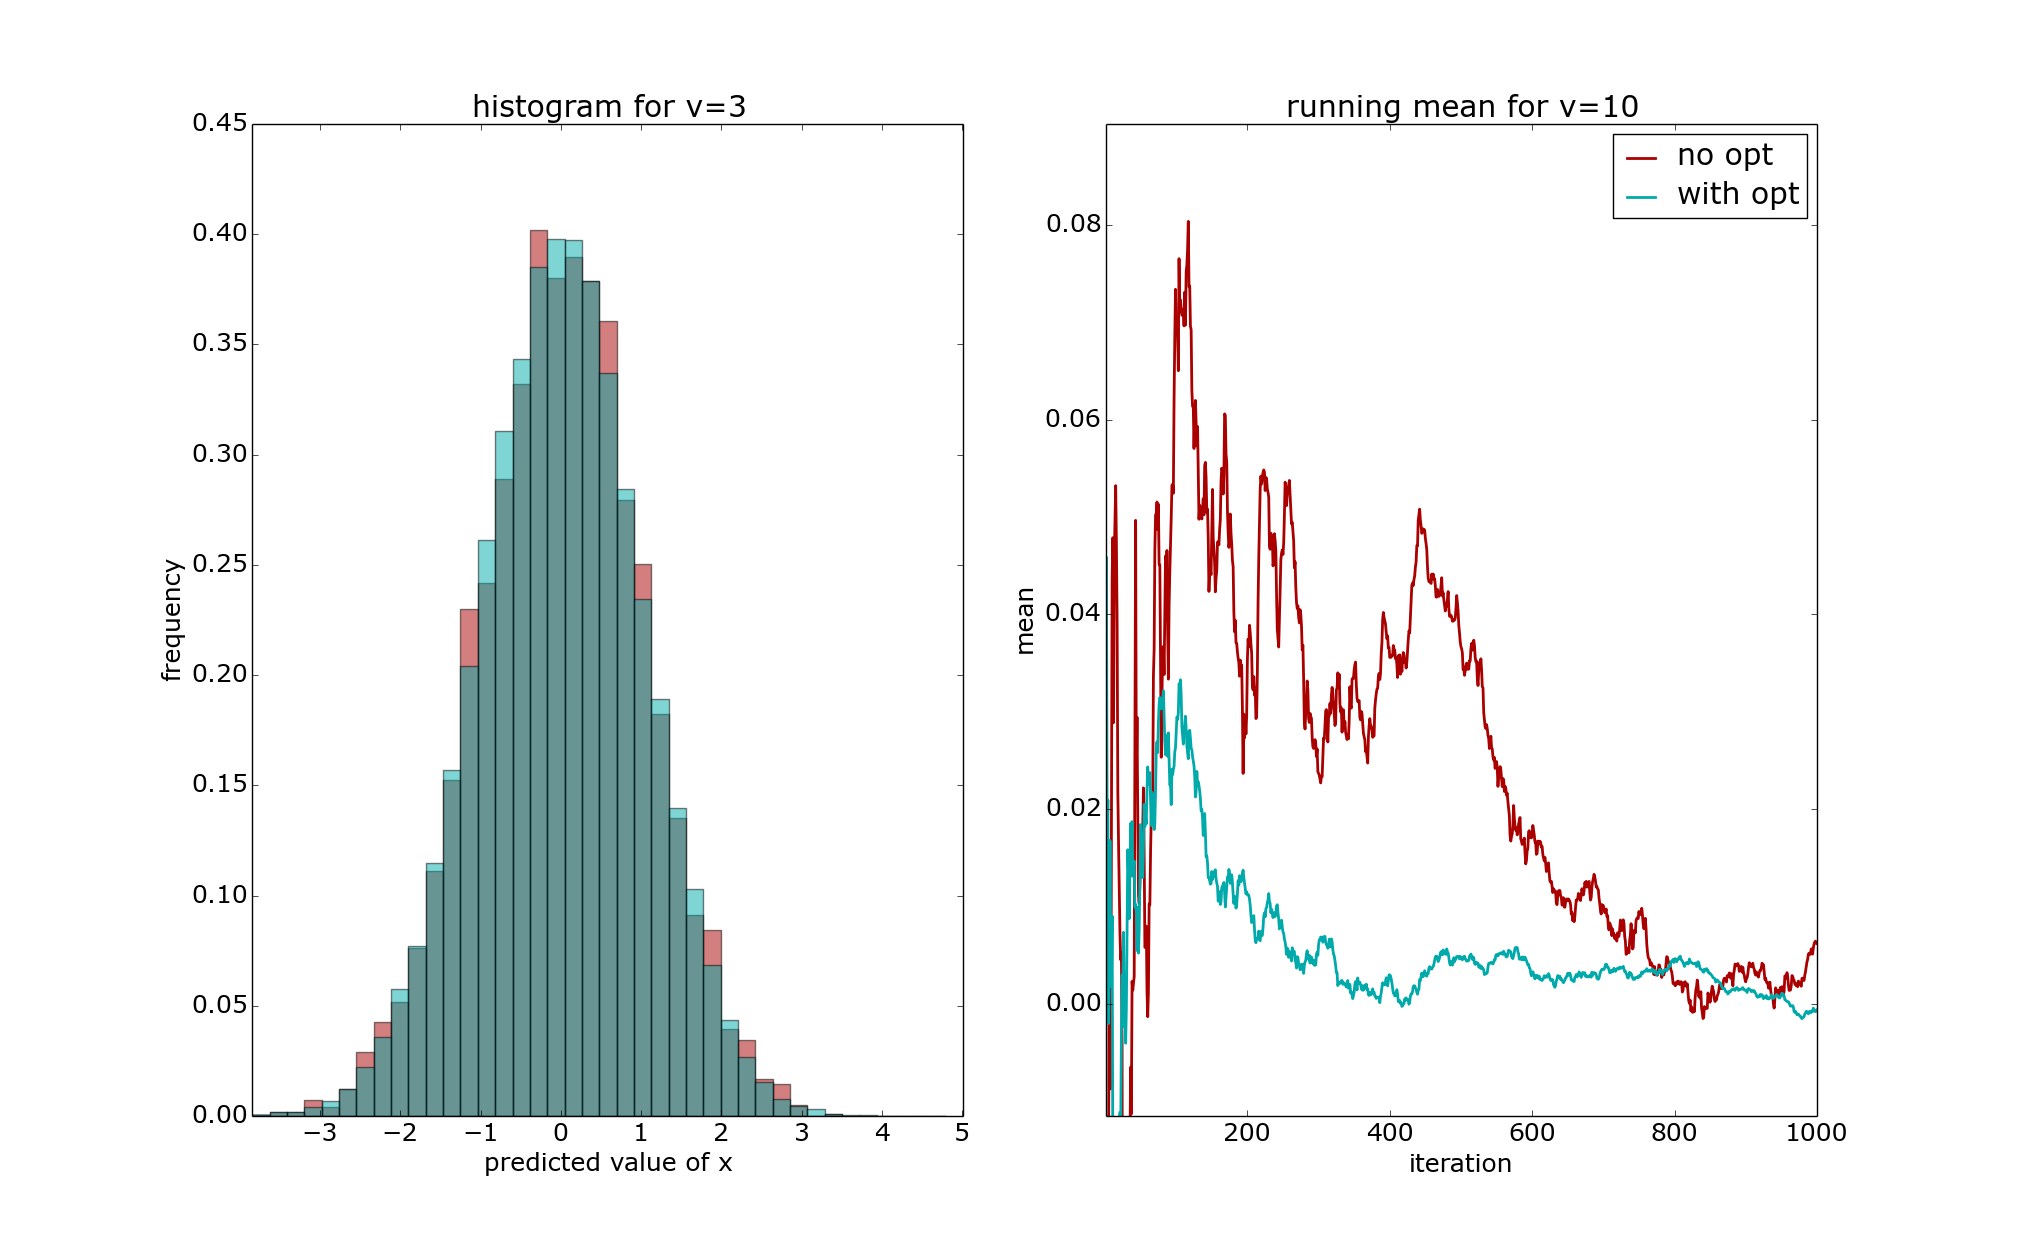
\includegraphics[width=16cm]{images/pushing_samples_back_1.png}}

This case demonstrates when the non-optimized program is still usable but the optimized program is superior in its mixing.

Now consider instead the case of \texttt{v = 10}, as shown in the next two graphs.

\centerline{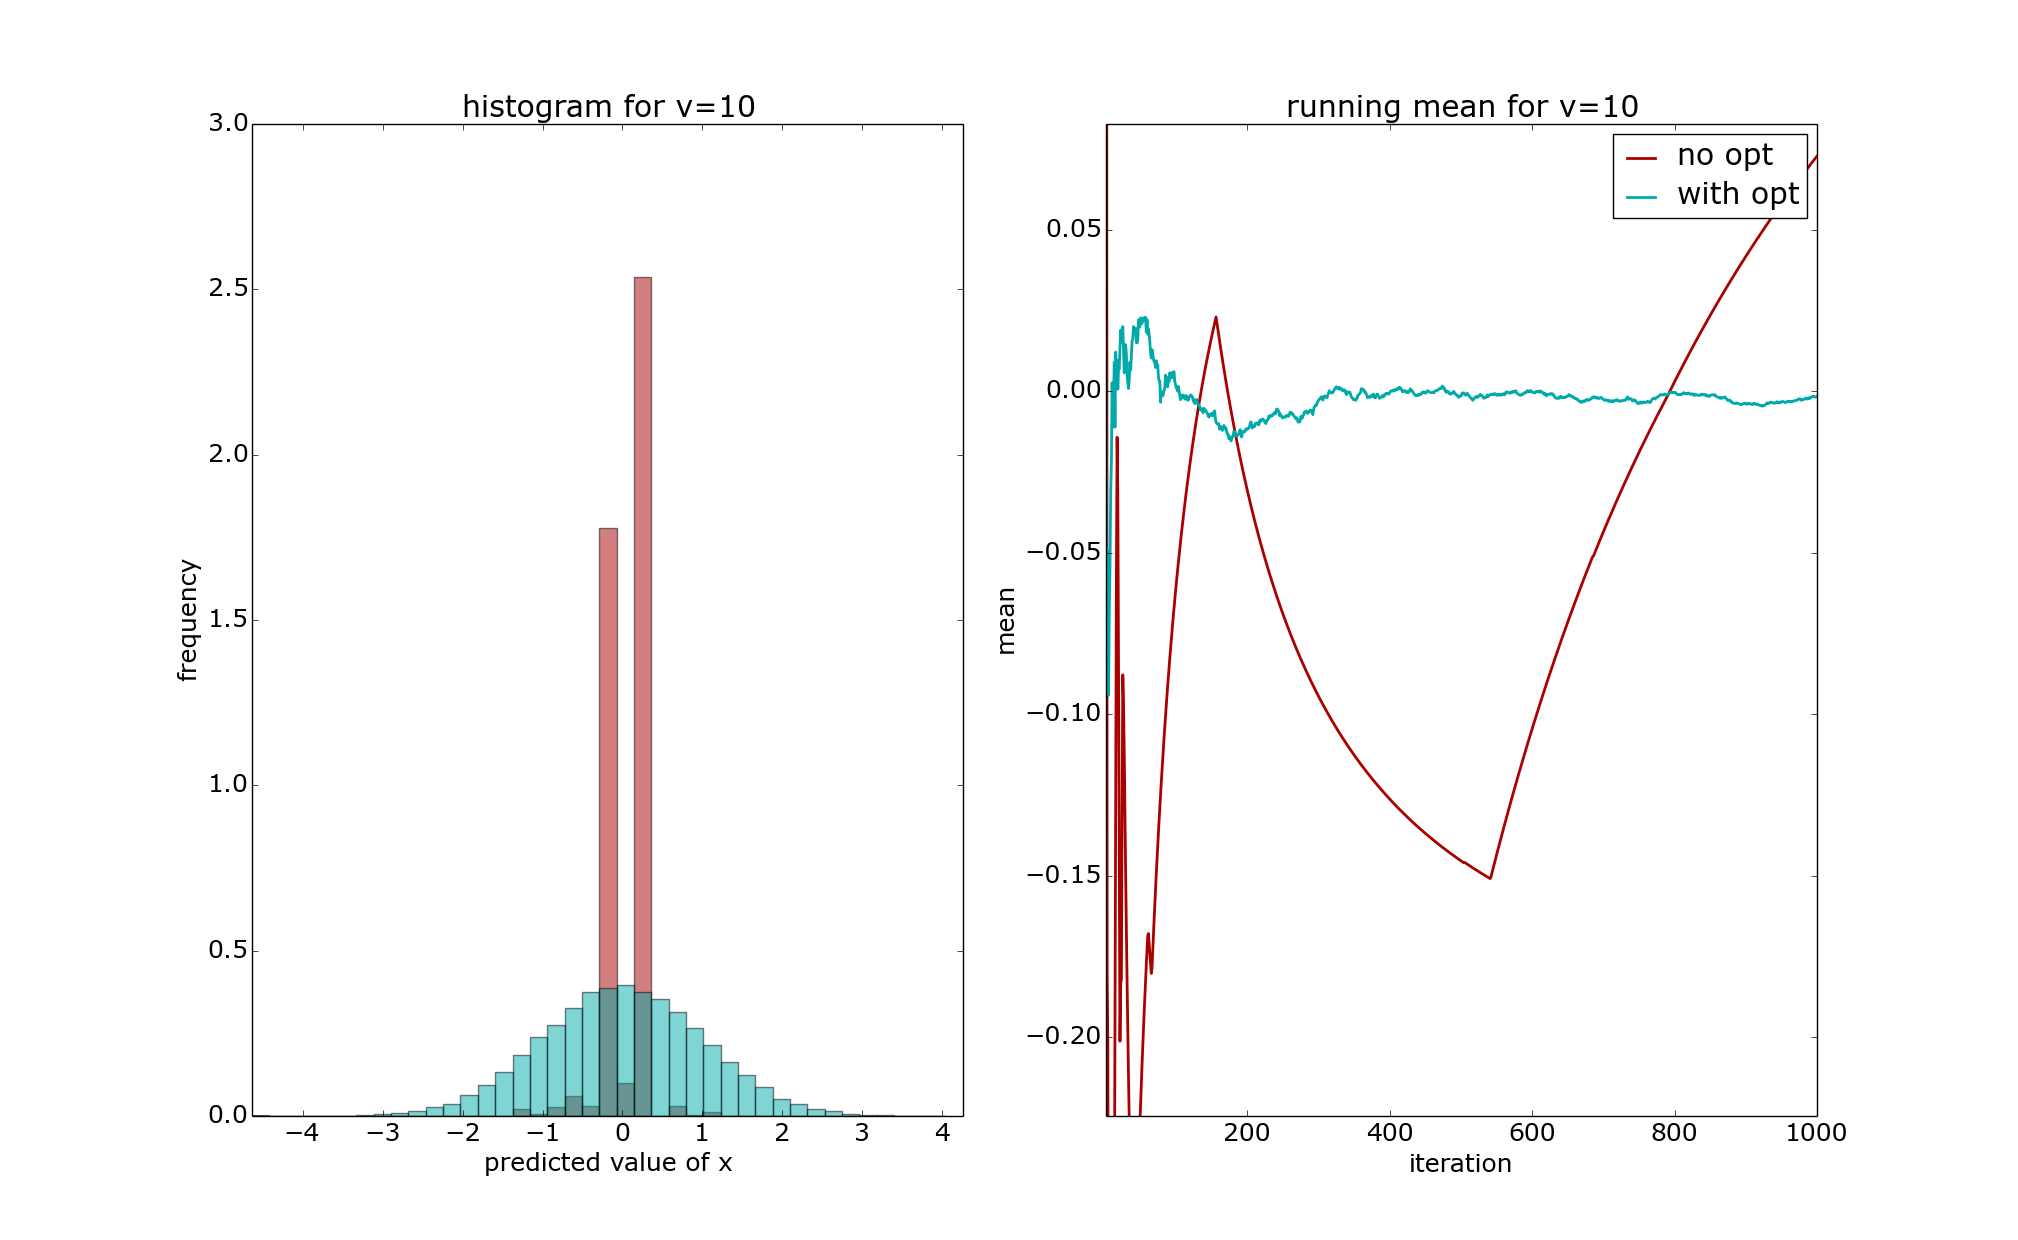
\includegraphics[width=16cm]{images/pushing_samples_back_2.png}}

This case demonstrates when the non-optimized program is completely useless however the optimized program is working exactly as well as it was before.



%    ########       ###### 
%    ##            ##    ##
%    ##                 ###
%     ######          ###  
%          ##       ###    
%    ##    ##  ##  ##      
%     ######   ##  ########

\subsection{Merging observes of the same distribution}

To test this optimization I used a program of the following form

\[
	\begin{array}{l}
		\texttt{[assume m (poisson 40)]} \\
		\texttt{[assume b 20]} \\
		\texttt{[observe (normal m b) 45]} \\
		\texttt{...} \\
		\texttt{[observe (normal m b) 45]} \\
		\texttt{[predict m]}
	\end{array}
\]
where the number of observe statements was varied. Programs of the above form were compiled with either no optimizations enabled or all optimizations enabled, then the resulting programs were run for 1000 iterations with 100 particles.

The following two graphs show running time against number of observes and mean value of the posterior distribution against number of observes.

\centerline{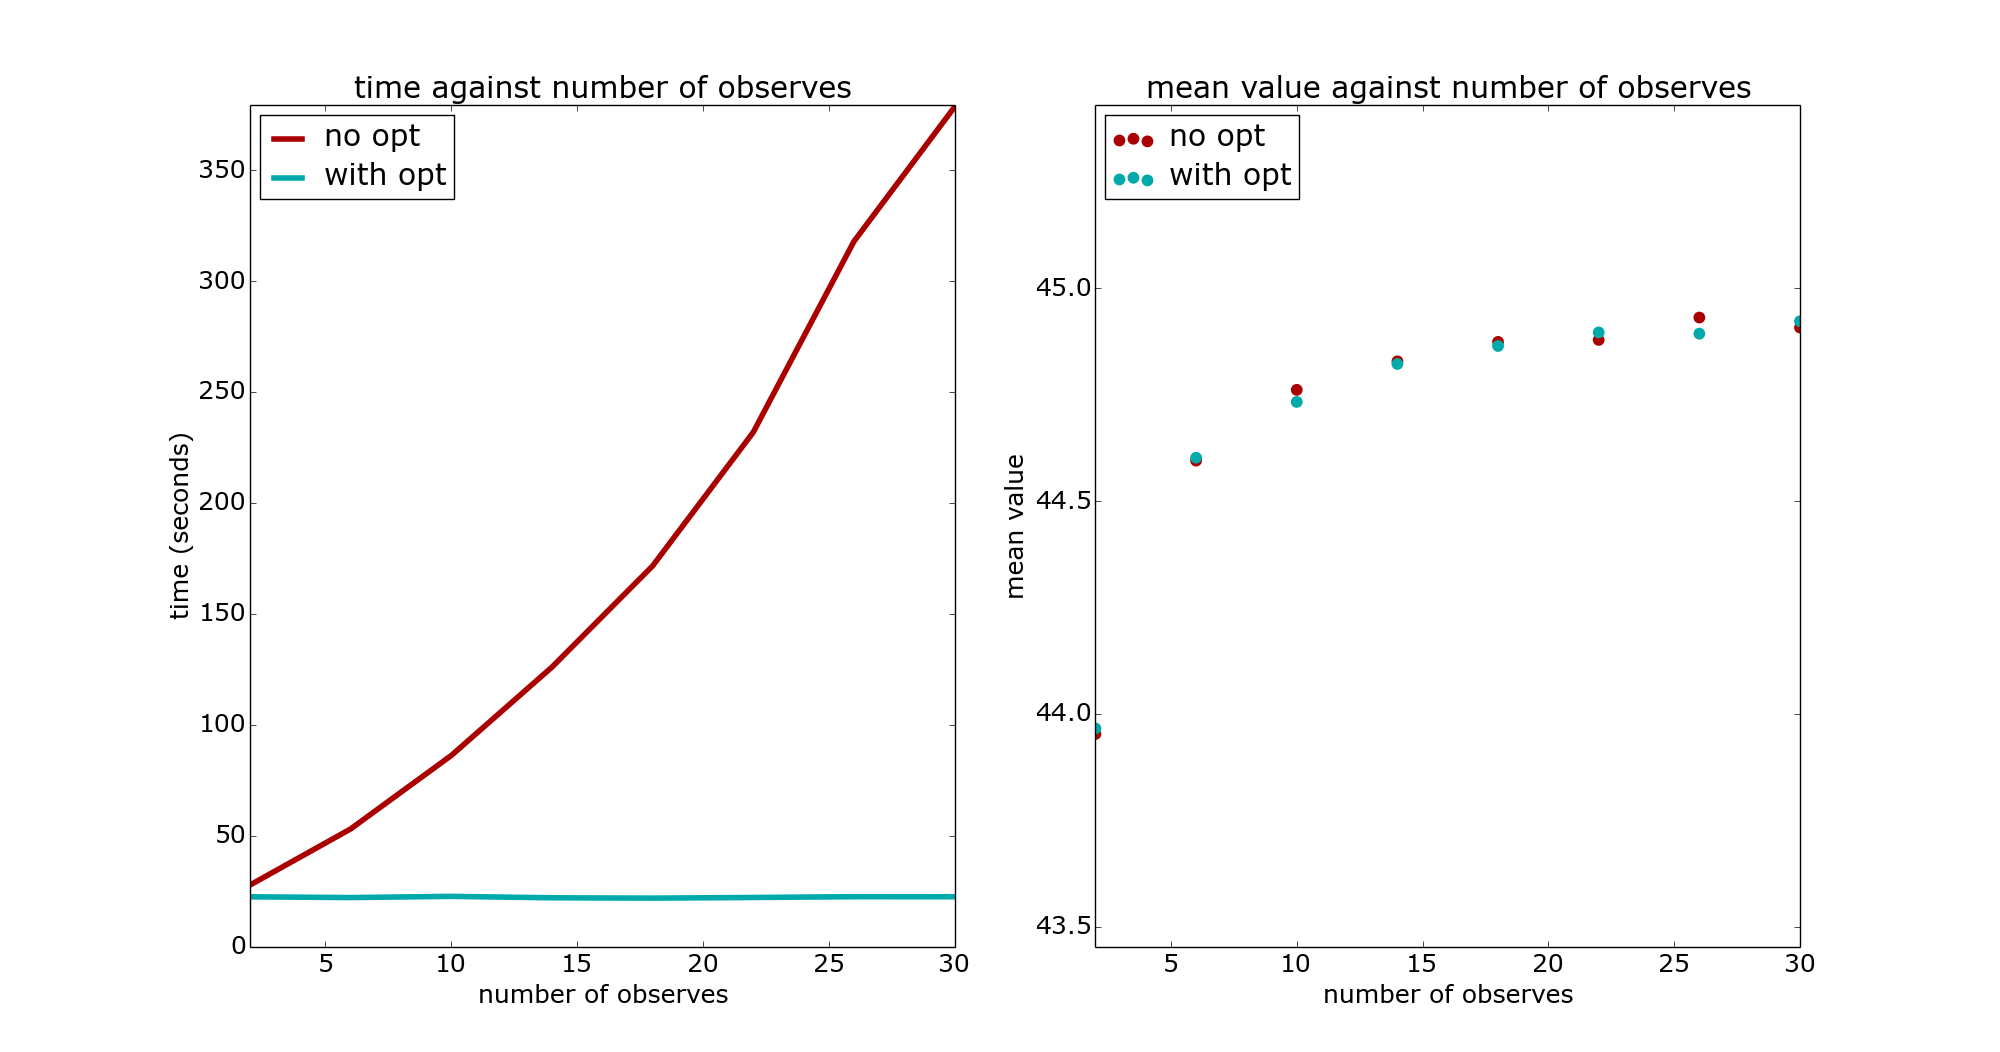
\includegraphics[width=16cm]{images/merging_observes_1.png}}

What you can see from these is firstly that the optimized and non-optimized programs give the same answer, but that the optimized program is far faster. Considering the complexity, it appears that the non-optimized program is close to linear in the number of observes, however the optimized program running time remains constant.

I will now investigate the \(n = 30\) case in more detail. These aspects can be seen in the following two graphs. The first graph shows the final posterior distribution. The second graph shows how the mean varies over time, so the value at t is the mean of the first t iterations.

\centerline{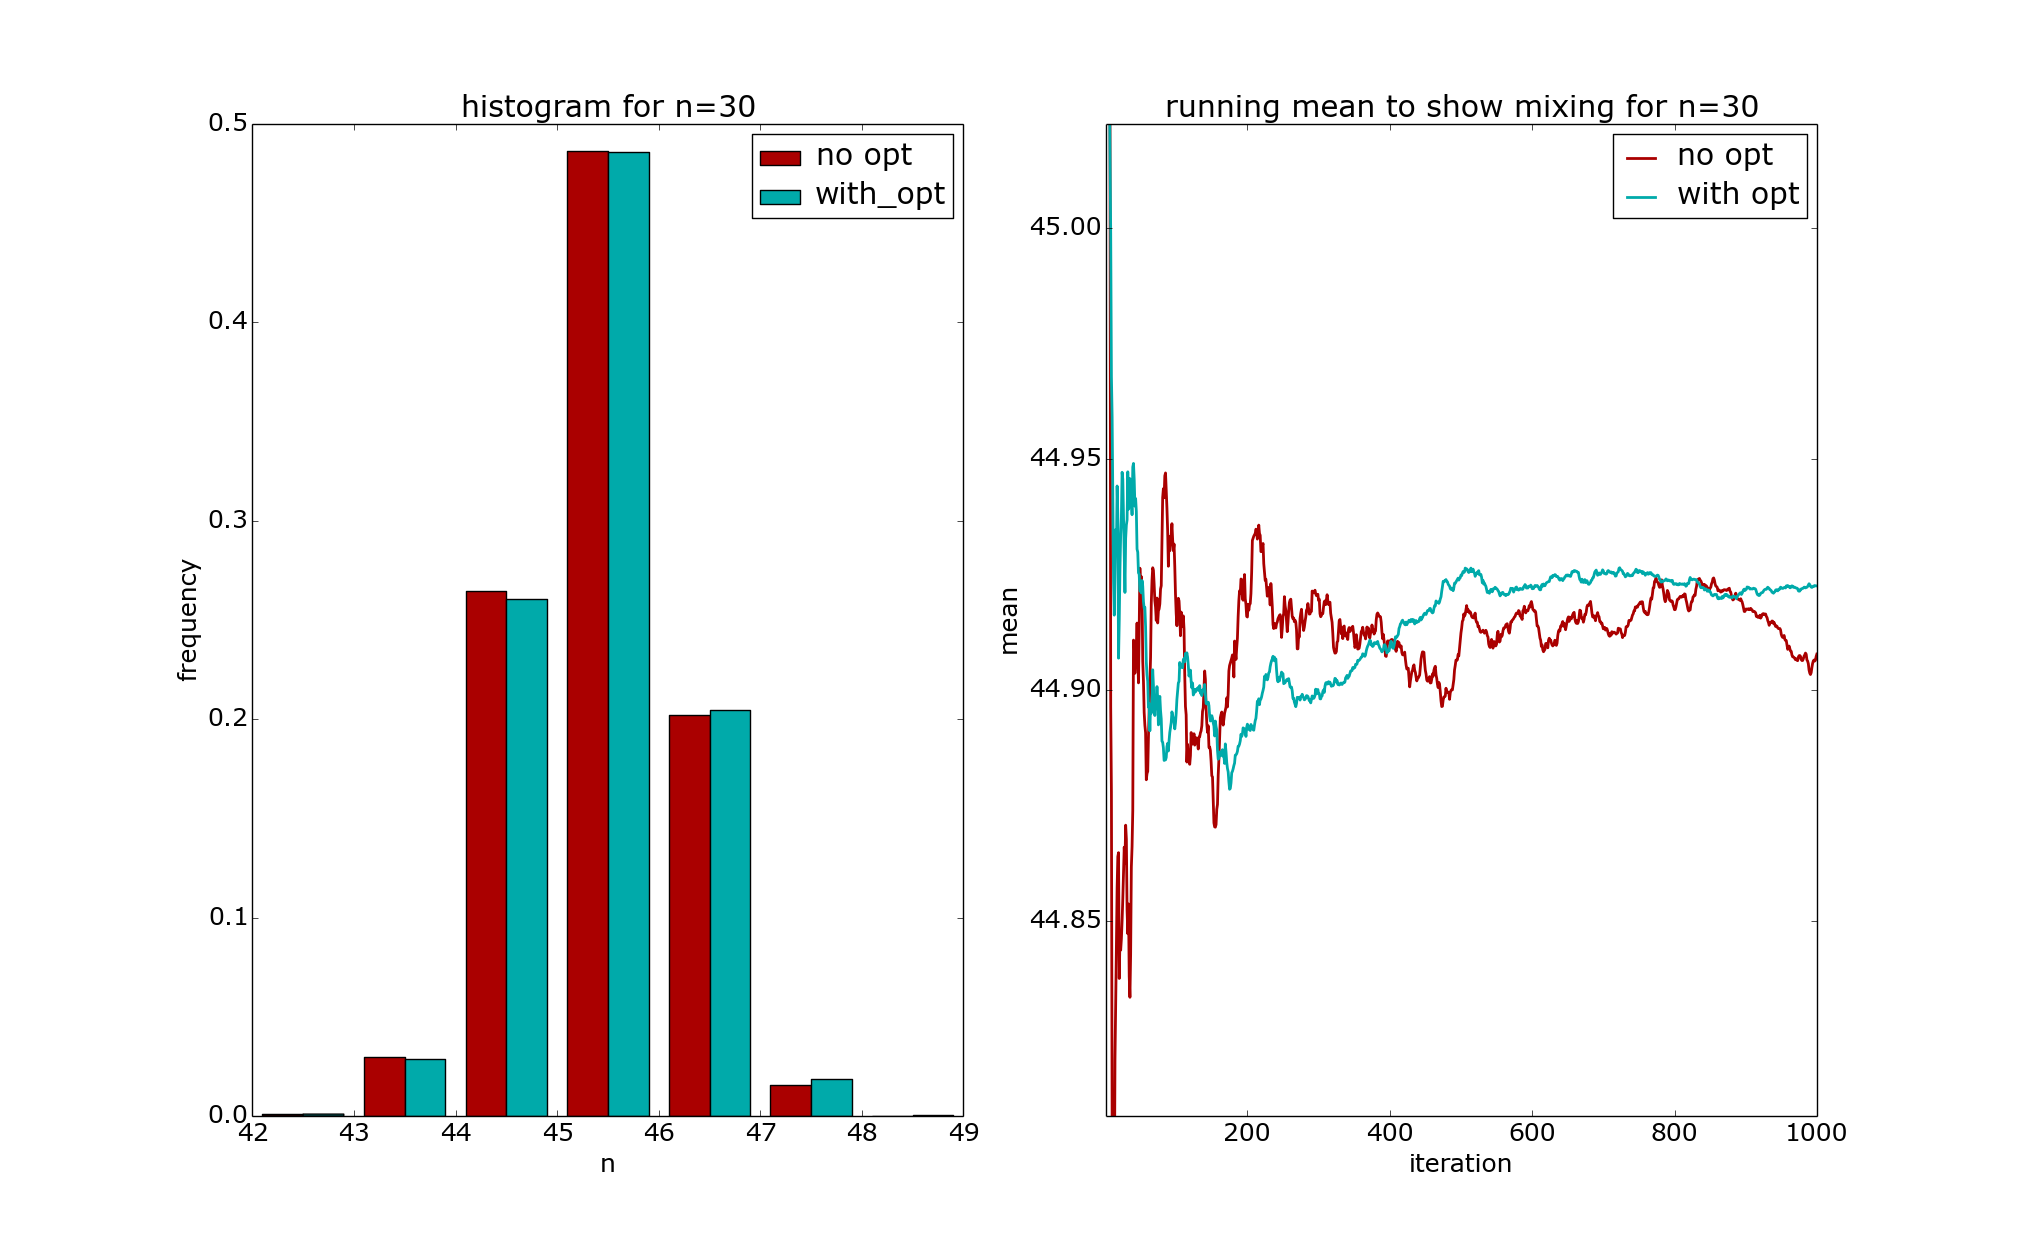
\includegraphics[width=16cm]{images/merging_observes_2.png}}

What you see from the first graph is again that the optimized and non-optimized programs give the same answer. Looking at the second graph it appears that the optimized program reaches it's final answer after around 600 iterations whilst the non-optimized program has still not converged satisfactorily after 1000 iterations, so at first glance the optimized program has better mixing, however I don't feel this is conclusive and would instead say that they perform roughly equally.



%    ########       ###### 
%    ##            ##    ##
%    ##                  ##
%     ######        ###### 
%          ##            ##
%    ##    ##  ##  ##    ##
%     ######   ##   ###### 

\subsection{Merging any consecutive observes}

To test this optimization I used a program of the following form

\[
	\begin{array}{l}
		\texttt{[assume m (normal 5 1)]} \\
		\texttt{[assume f (lambda () -> Num m)]} \\
		\texttt{[observe (normal (f) 0.1) 4]} \\
		\texttt{...} \\
		\texttt{[observe (normal (f) 0.1) 4]} \\
		\texttt{[predict m]}
	\end{array}
\]
where the number of observe statements was varied. Programs of the above form were compiled with either no optimizations enabled or all optimizations enabled, then the resulting programs were run for 1000 iterations with 100 particles.

The following two graphs show running time against number of observes and mean value of the posterior distribution against number of observes.

\centerline{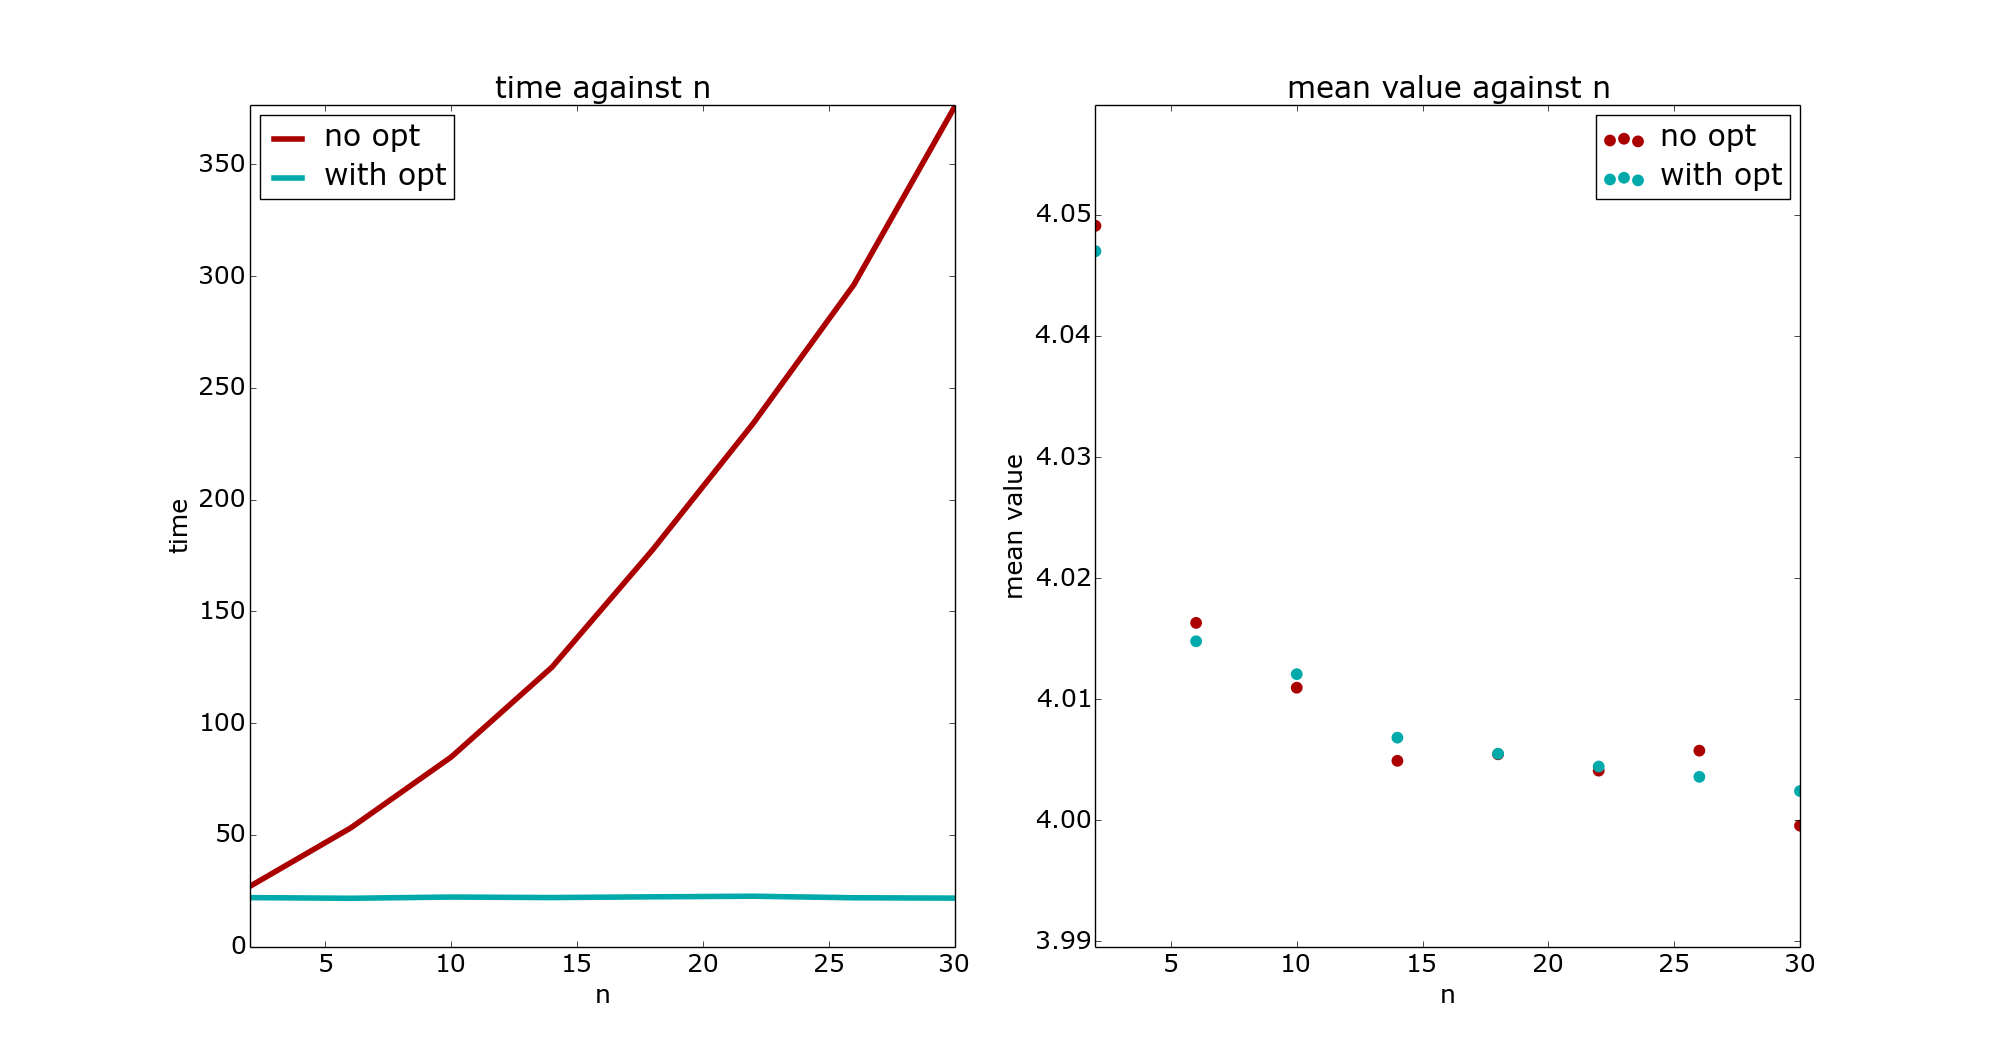
\includegraphics[width=16cm]{images/merging_consecutive_observes_1.png}}

What you can see from these is firstly that the optimized and non-optimized programs give the same answer to within an acceptable margin, but again that the optimized program is far faster. Considering the complexity, it again appears that the non-optimized program is close to linear in the number of observes, however the optimized program running time remains constant.

I will now investigate the \(n = 30\) case in more detail. These aspects can be seen in the following two graphs. The first graph shows the final posterior distribution. The second graph shows how the mean varies over time, so the value at t is the mean of the first t iterations.

\centerline{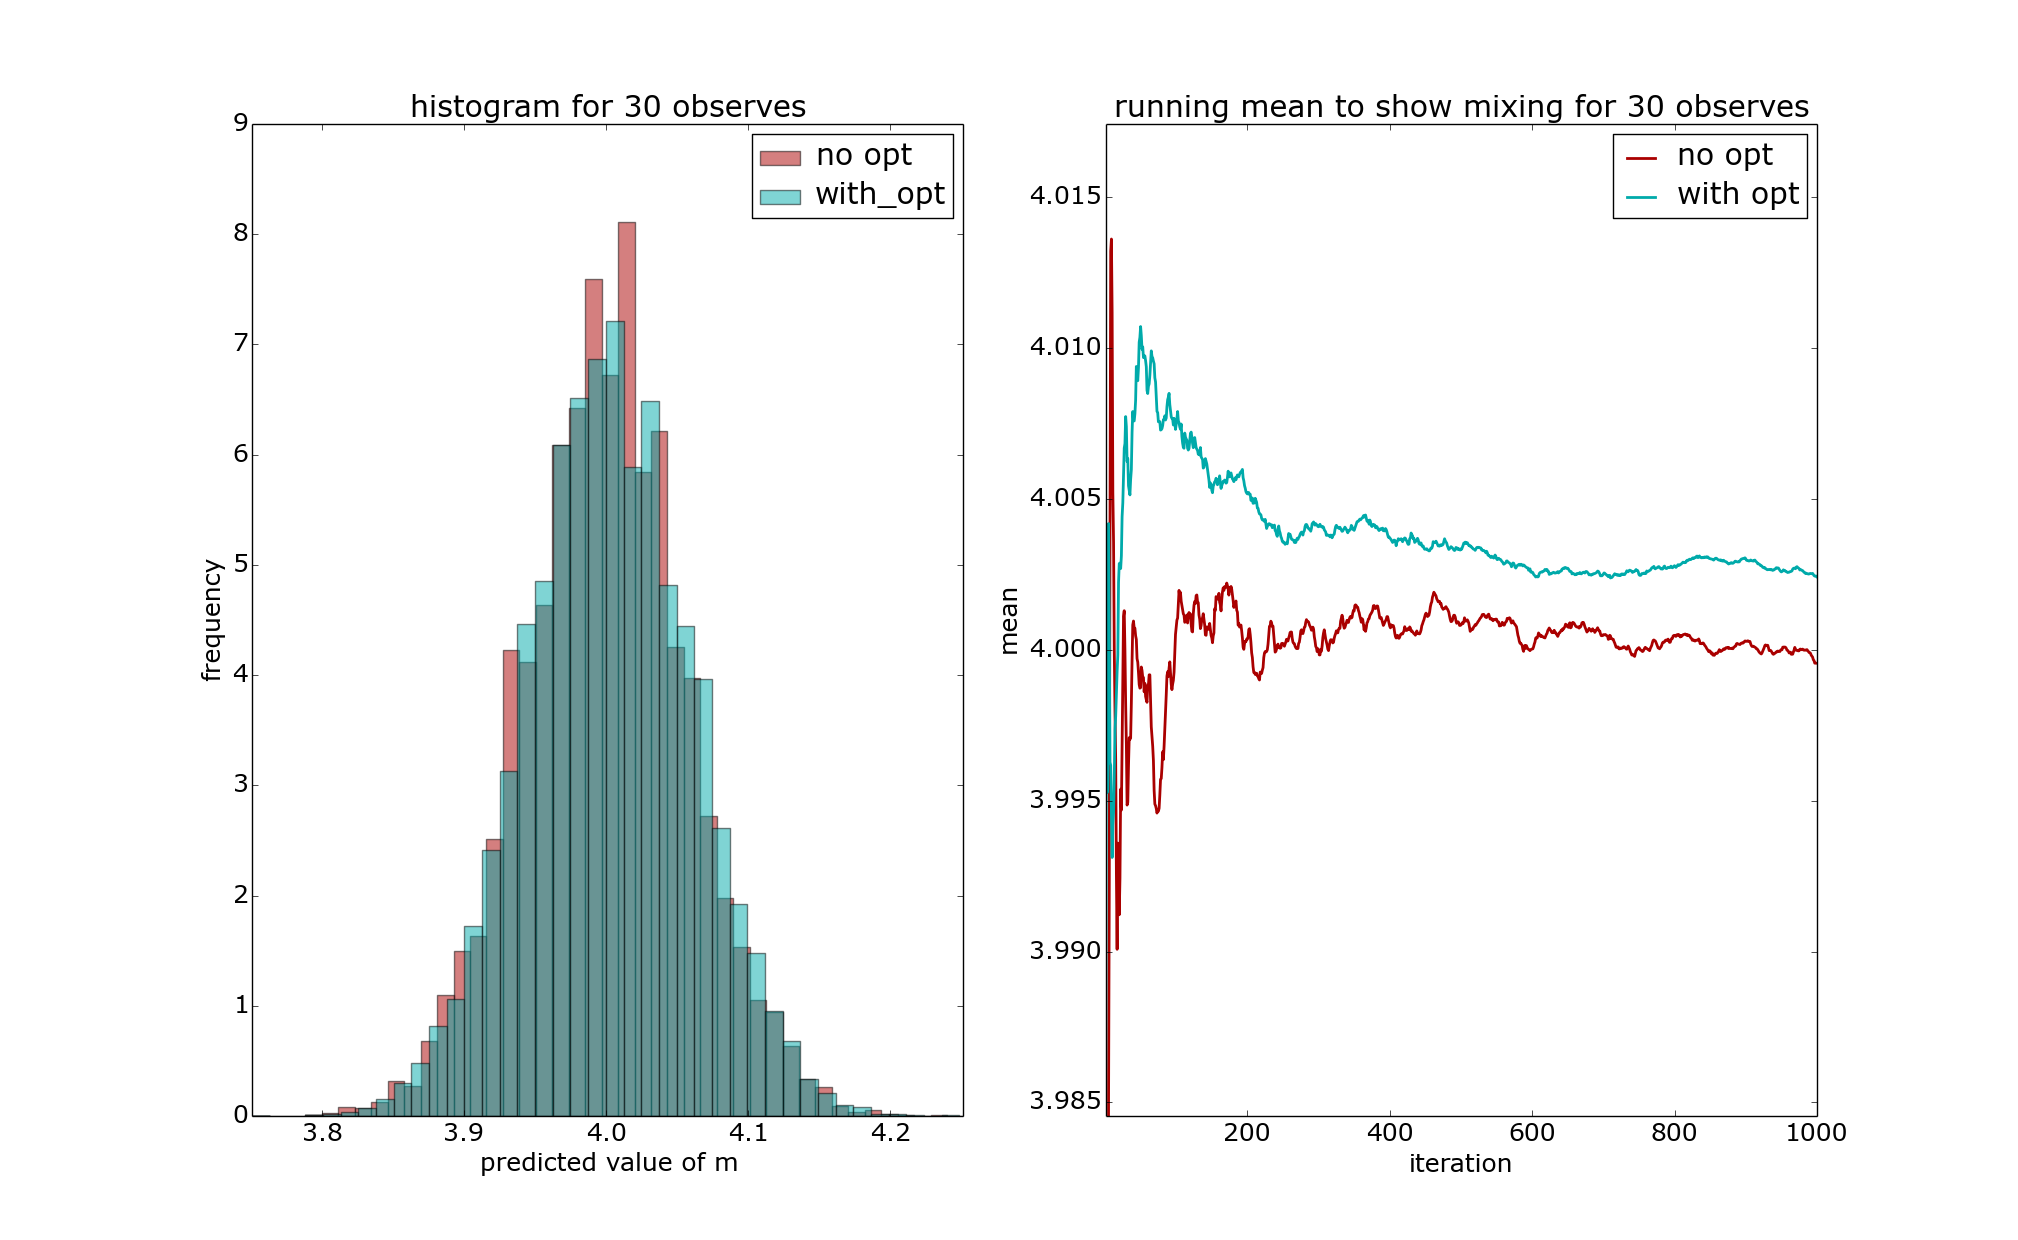
\includegraphics[width=16cm]{images/merging_consecutive_observes_2.png}}

What you see from the first graph is again that minus a bit or noise the optimized and non-optimized programs give the same answer. Looking at the second graph they appear to have similar levels of mixing, that is they both approach their final mean value of posterior distribution at the same rate.



%    ########          ### 
%    ##               #### 
%    ##              ## ## 
%     ######        ##  ## 
%          ##      ########
%    ##    ##  ##       ## 
%     ######   ##       ## 

\subsection{Removing observes}

To test this optimization I used a program of the following form

\[
	\begin{array}{l}
		\texttt{[assume m (normal 10 4)]} \\
		\texttt{[observe (normal m 0.1) 15]} \\
		\texttt{...} \\
		\texttt{[observe (normal m 0.1) 15]} \\
		\texttt{[predict m]}
	\end{array}
\]
where the number of observe statements was varied. Programs of the above form were compiled with either no optimizations enabled or all optimizations enabled, then the resulting programs were run for 1000 iterations with 100 particles.

The following two graphs show running time against number of observes and mean value of the posterior distribution against number of observes.

\centerline{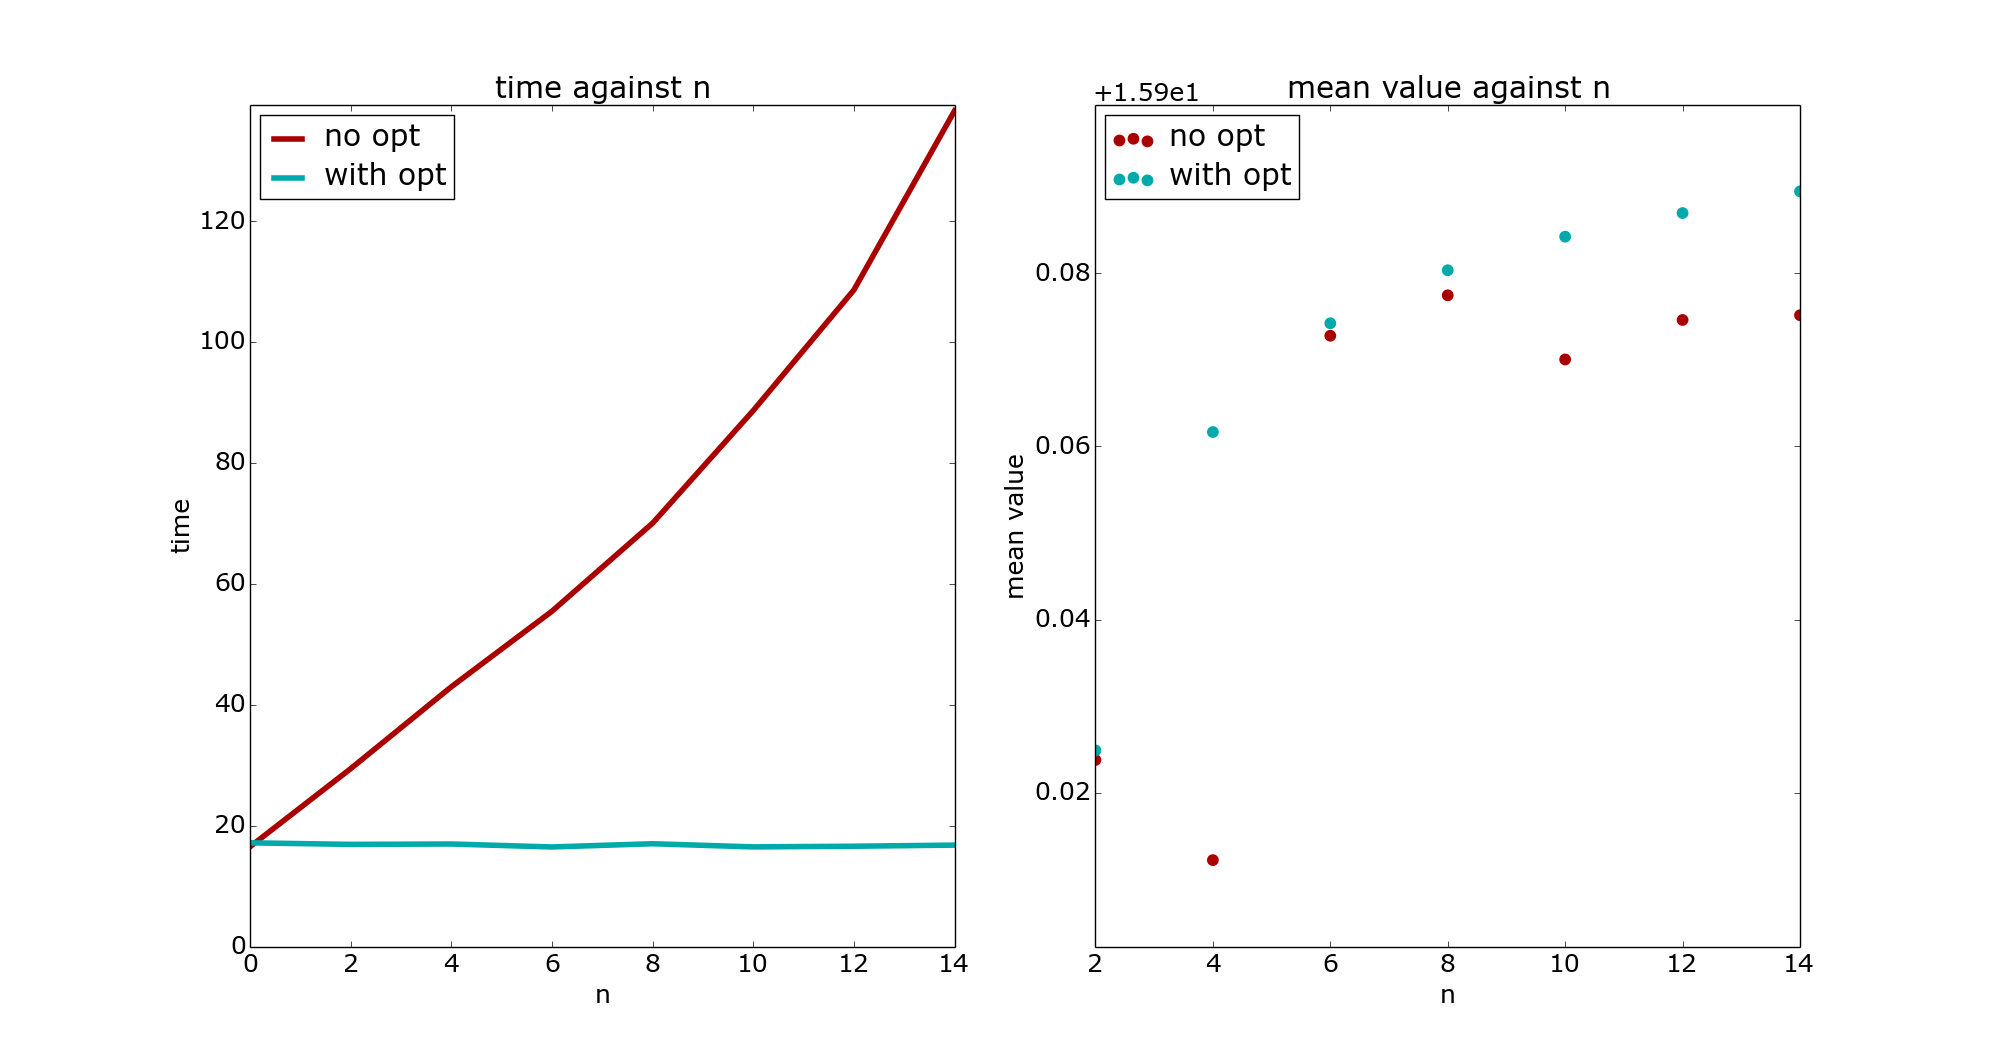
\includegraphics[width=16cm]{images/removing_observes_1.png}}

What you can see here is firstly that the optimized program is far faster than the non-optimized one, and the optimized program gives a sensible and correct answer whereas the non-optimized programs are much less consistent. Considering complexity, it again appears that the non-optimized program is close to linear in the number of observes, however the optimized program running time remains constant.

I will now show the extend to which the non-optimized programs fail to give usable output, looking at the posterior distribution of each one and showing how it deteriorates as the number of observes increases. Consider the following set of graphs.

\centerline{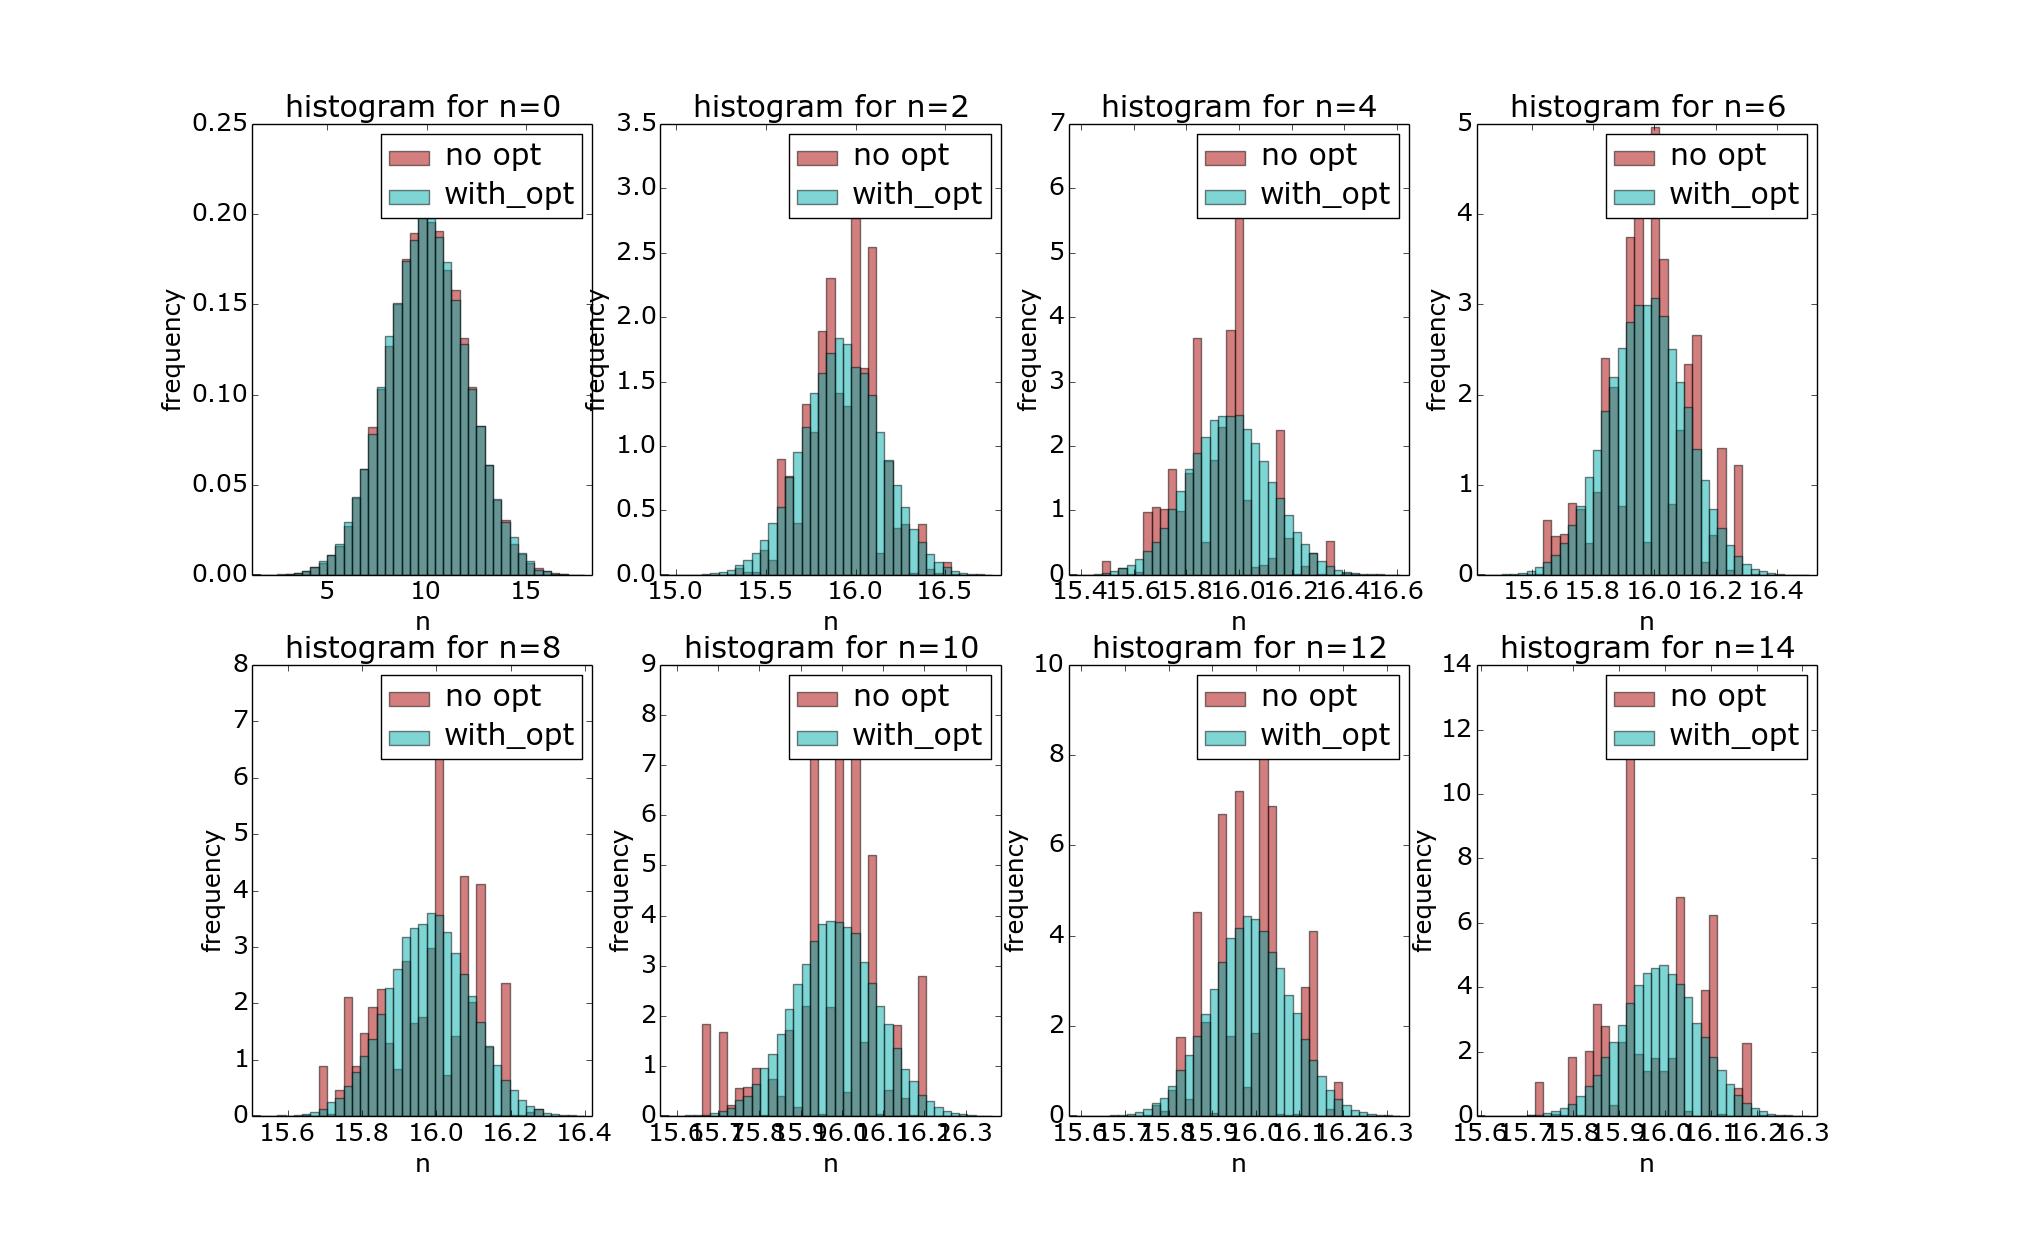
\includegraphics[width=16cm]{images/removing_observes_2.png}}

What you can see here is that the optimized program gives a perfect normal distribution every time, in fact we could have run far fewer than 1000 iterations and still achieved a good distribution. However, the non-optimized program's distributions are much less clean and if we were to increase the number of observes more or move the observed value further from the value \texttt{m} then the distributions would deteriorate even more. The non-optimized program is not even usable except in easy cases, so this optimization actually opens whole new areas of program that can be written rather than just making things faster.

\end{document}
